%%%%%%%%%%%%%%%%%%%%%%%%%%%%%%%%%%%%%%%%%
% University/School Laboratory Report
% LaTeX Template
% Version 3.1 (25/3/14)
%
% This template has been downloaded from:
% http://www.LaTeXTemplates.com
%
% Original author:
% Linux and Unix Users Group at Virginia Tech Wiki 
% (https://vtluug.org/wiki/Example_LaTeX_chem_lab_report)
%
% License:
% CC BY-NC-SA 3.0 (http://creativecommons.org/licenses/by-nc-sa/3.0/)
%
%%%%%%%%%%%%%%%%%%%%%%%%%%%%%%%%%%%%%%%%%

%----------------------------------------------------------------------------------------
%	PACKAGES AND DOCUMENT CONFIGURATIONS
%----------------------------------------------------------------------------------------

\documentclass{article}

% Notations
\usepackage{amsmath} % Required for some math elements
\usepackage{amssymb}
\usepackage{siunitx} % Provides the \SI{}{} and \si{} command for typesetting SI units, sudo apt -y install texlive-science

% Citations
\usepackage[backend=bibtex,style=numeric]{biblatex} % sudo apt-get install texlive-bibtex-extra biber
\addbibresource{../../bibtex/bibtex.bib}
\usepackage{hyperref}
\usepackage{url} % Provides better formatting of URLs.
\usepackage{csquotes}

% Figures
\usepackage{graphicx} % Required for the inclusion of images
\usepackage{float} % float or non floating figures options

% General appearance/geometry
\usepackage[legalpaper, portrait, margin=1in]{geometry}

% Text appearance
\usepackage{ragged2e}
\RaggedRight
\setlength\parindent{0pt} % Removes all indentation from paragraphs
\renewcommand{\labelenumi}{\alph{enumi}.} % Make numbering in the enumerate environment by letter rather than number (e.g. section 6)

%\usepackage{times} % Uncomment to use the Times New Roman font
%^\circ for the degree sign ' or ^\prime for the minute mark, and '' for seconds

%----------------------------------------------------------------------------------------
%	DOCUMENT INFORMATION
%----------------------------------------------------------------------------------------

\title{Methodology notes} % Title

\author{Tobbey McNamara} % Author names
%tobbey.mcnamara@gmail.com, tobbey.mcnamara@gmail.com }} % Author email addresses

\begin{document}


\maketitle % Insert the title, author and date
\begin{figure}[H]
\centering
  
\includegraphics[scale=1]{../../figures/shelyak-transparent.png}\\ % University/lab logo
\end{figure}


% If you wish to include an abstract, uncomment the lines below
\begin{abstract}
This internal document aims at presenting definitions and description of various methodological processes.
\end{abstract}

%----------------------------------------------------------------------------------------
%	SECTION 1
%----------------------------------------------------------------------------------------

\section{Electronic sensor calibration}
  \subsection{Definitions}
    \subsubsection{ADU}
    This acronym stands for Analog to Digital Unit, also known as digital count.
    \subsubsection{Dark current}
    \subsubsection{Amp glow}
    \subsubsection{Defective pixel}
    Usually, defective pixels from a sensor are classified into 5 main classes:
    \begin{itemize}
     \item Hot pixels
     \item Warm pixels
     \item Cold pixels
     \item Dead pixels
    \end{itemize}
    
    \subsubsection{Signal to noise ratio} Signal to noise ratio is often measured in terms of PSNR (Point Signal to Noise Ratio).

    
  \subsection{Sensor offset}
    offset map 
    
  \subsection{Sensor Bias}    
    
  \subsection{Sensor dark current}
    dark current table at different temperature and different gain
    
    From a statistical point of view, one of the more important role of dark calibration is to reduce the variance due to an additive deterministic signal coming from the sensor itself, whether there is incident light applied on it or not.
    It is generally admitted that, on cmos sensor, most of the deterministic signal that can be reproduced in similar temperature/gain/exposure time is due to dark current, and/or amp glow.
    
    The dark calibration process can then be divided into two parts:
    \begin{itemize}
     \item Dark library acquisition
     \item Dark signal substraction
    \end{itemize}

    \subsection{Dark library acquisition} The role of this task is to acquire, for each condition, a set of images while the sensor is not exposed to any light. A condition in that case is defined by 3 parameters: (Electronic Gain, Sensor Temperature, Exposure time).
    Of course, in order for this library to be created, on needs to choose a reasonable sampling of this 3d space to keep the overall process feasible in practice.
    
    \paragraph{Signal to noise ratio} It is of crucial importance to have the best possible signal to noise ratio on the dark image from the dark signal library. Indeed, as the deterministic signal is meant to be substracted from the image, we surely don't want to introduce more variance due to noise in the dark reference, that there was initially in the image to be corrected.

    \paragraph{Dark signal estimation / parametrization}
    Depending on the sampling, one might be interested in implementing an interpolation method that would help to guess what was the actual dark signal in between samples from the 3d space.
    There are three main classes of methods to estimate dark signal for a given configuration:
    \begin{itemize}
     \item Model based interpolation: Given a coordinate $(g,t,e)$ in the (gain, temperature, exposure time) 3-D space, and a set of images from the dark library $l$ one can use an arbitrary interpolation method $dark(g,t,e,l)$ to generate a synthetic dark image. In the case of a linear interpolation method, one can probably write:
     
     \begin{align*}
      dark(g,t,e,l) = \frac{1}{normalisation} \sum_{i \in l} coefficient((g,t,e), coordinates(i)) dark_i 
     \end{align*}

     It is important do understand that the $coefficient$ function can be arbitrarily complex. One can either use a naive bilinear interpolation method, or eventually try to model the behavour of the $dark_i$ vector with a more complex model, like multivariate function (2D or 3D most likely) of one or multiple dark reference or synthetic dark reference models.
     
     \item Variance based interpolation. Another possibility is to try to fit directly one or multiple dark images reference from the library to an acquisition, given a cost function. In particular, we can eventually get back to the very definition of dark calibration method. Its role is to reduce the variance due to deterministic sensor signal, hence we can use the overall image variance as a cost function to be minimized over the space of interpolation parameters. One can for instance choose 4 reference images $r_0,r_1,r_2,r_3$, closest to the current $(g,t,e)$ coordinates, and try to fit a simple linear model with a least square formulation:
     \begin{align*}
      synth_{dark} &= \sum_{i=0}^{3} a_i r_i \qquad \text{s.t} \\
      \begin{pmatrix} r_0\\ r_1\\ r_2\\ r_3\end{pmatrix} &= \underset{r \in \mathbb{R}^4}{argmin} \| \left(image - \sum_{i=0}^{3} a_i r_i \right) - \left( \frac{1}{card(image)} \left(image_i - \sum_{i=0}^{3} a_i (r_i)_j \right) \cdot \vec{1}_{card(image)} \right) \vec{1}_{card(image)} \|_2^2 \\
      &= \underset{r \in \mathbb{R}^4}{argmin} \| aaaaaaa \|_2^2
     \end{align*}

    \end{itemize}

    It is generally admitted, that dark signal might vary non linearly from one gain to another


    There are actually multiple ways to do that:
    \begin{itemize}
     \item 
    \end{itemize}
    
    \paragraph{Variance based dark optimization}
    \begin{align*}
	synth_{dark} &= \sum_{i=0}^{3} a_i r_i \qquad \text{s.t} \\
	      \begin{pmatrix} a_0\\ a_1\\ a_2\\ a_3\end{pmatrix} &= \underset{a \in \mathbb{R}^4}{argmin} \| \left(image - \sum_{i=0}^{3} a_i r_i \right) - \left( \frac{1}{card(image)} \left(image_i - \sum_{i=0}^{3} a_i (r_i)_j \right) \cdot \vec{1}_{card(image)} \right) \vec{1}_{card(image)} \|_2^2
    \end{align*}

    Lets write for simplicity:
    * $card(image) = c$ a scalar standing for the total number of pixels in the image
    * $\begin{pmatrix} a_0\\ a_1\\ a_2\\ a_3\end{pmatrix} = \vec{x}$ the actual vector of weighting coefficients
    * $\begin{pmatrix} -\vec{r_0} & -\vec{r_1} & -\vec{r_2} & -\vec{r_3}\end{pmatrix} = A$ the matrix containing the candidate dark images.
    * $image = -\vec{y}$ The vector $image$ representing the actual image from which we would like to remove dark signal

    We can now rewrite
    \begin{align*}
	      x &= \underset{x \in \mathbb{R}^4}{argmin} \| A\vec{x}-\vec{y} - \left(\frac{1}{c} (A\vec{x}-\vec{y})\cdot\vec{1}_{c} \right) \vec{1}_{c} \|_2^2 \\
    \end{align*}

    To simplify this further, we would also like to identify 
    * $ A\vec{x}-\vec{y}$ as $\vec{v}$
    to make the expression simpler to develop:
    \begin{align*}
	      x &= \underset{x \in \mathbb{R}^4}{argmin} \qquad \| A\vec{x}-\vec{y} - \left( \frac{1}{c} (A\vec{x}-\vec{y})\cdot\vec{1}_{c}\right) \vec{1}_{c} \|_2^2 \\
	      &= \underset{x \in \mathbb{R}^4}{argmin} \qquad \| \vec{v} - \left( \frac{1}{c} (\vec{v}\cdot\vec{1}_{c}) \right) \vec{1}_{c} \|_2^2 \\
	      &= \underset{x \in \mathbb{R}^4}{argmin} \qquad v^{T}v + \frac{1}{c^2} (v^{T}1_{c})^2 (1_{c}^{T}1_{c}) - \frac{2}{c} (v^{T}1_{c})(v^{T}1_{c}) \\
	      &= \underset{x \in \mathbb{R}^4}{argmin} \qquad v^{T}v + \frac{1}{c^2} (1_{c}^{T}1_{c} - 2c)(v^{T}1_{c})^2 \\
	      &= \underset{x \in \mathbb{R}^4}{argmin} \qquad v^{T}v + \frac{1}{c^2} (c - 2c)(v^{T}1_{c})^2 \qquad \text{because } \; 1_{c}^{T}1_{c} = c\\
	      &= \underset{x \in \mathbb{R}^4}{argmin} \qquad v^{T}v - \frac{1}{c} (v^{T}1_{c})^2 \\          
    \end{align*}

    Lets now plug back in our slightly more complex expression:

    \begin{align*}
	      x &= \underset{x \in \mathbb{R}^4}{argmin} \qquad v^{T}v - \frac{1}{c} (v^{T}1_{c})^2 \\
	      &= \underset{x \in \mathbb{R}^4}{argmin} \qquad (Ax-y)^{T}(Ax-y) - \frac{1}{c} \left( (Ax-y)^{T}1_{c} \right)^2 \\
	      &= \underset{x \in \mathbb{R}^4}{argmin} \qquad x^{T}A^{T}Ax + y^{T}y -2y^{T}Ax - \frac{1}{c} \left( (1_{c}^{T}Ax-1_{c}^{T}y)^2 \right) \\
	      &= \underset{x \in \mathbb{R}^4}{argmin} \qquad x^{T}A^{T}Ax + y^{T}y -2y^{T}Ax - \frac{1}{c} \left( x^{T}(A^{T}1_{c}(A^{T}1_{c})^{T})x + (1_{c}^{T}y)^2 -2(1_{c}^{T}y)1_{c}^{T}Ax ) \right) \\
	      &= \underset{x \in \mathbb{R}^4}{argmin} \qquad \underbrace{x^{T}A^{T}Ax -\frac{1}{c} x^{T}(A^{T}1_{c}(A^{T}1_{c})^{T})x}_{\text{Quadratic part}} \; + \; \underbrace{-2y^{T}Ax +\frac{2}{c}(1_{c}^{T}y)1_{c}^{T}Ax )}_{\text{Linear part}} \; + \; \underbrace{y^{T}y -\frac{1}{c}(1_{c}^{T}y)^2}_{Constant part} \\
    \end{align*}

    This expression looks pretty familiar, it simply looks like the sum of two quadratic problems.
    Proving convexity then amount to prove that Hessian is definite positive.

    \begin{align*}
	H = A^{T}A - \frac{1}{c} A^{T}1_{c}(A^{T}1_{c})^{T}
    \end{align*}

    We see directy that $A^{T}A$ is symmetric, so we should be fine with semi definiteness beside trivial case (A=0). Lets take a closer look at this other weird expression

    \begin{align*}
	A^{T}1_{c}(A^{T}1_{c})^{T}
    \end{align*}

    We decided to write that matrix this way because it shows that it can be rewritten $M^{T}M$ by identifying $M=(A^{T}1_{c})^{T}$. Hence it was easy to prove that the matrix is symmetric, hence $H$ is symmetric, then the Hessian of the problem is at least positive semi definite.

    Thanks to basic matrix calculus rule, we can simply differentiate now the general coest function expression in $x$:

    \begin{align*}
	      f(x) &= \underbrace{x^{T}A^{T}Ax -\frac{1}{c} x^{T}(A^{T}1_{c}(A^{T}1_{c})^{T})x}_{\text{Quadratic part}} \; + \; \underbrace{-2y^{T}Ax +\frac{2}{c}(1_{c}^{T}y)1_{c}^{T}Ax )}_{\text{Linear part}} \; + \; \underbrace{y^{T}y -\frac{1}{c}(1_{c}^{T}y)^2}_{Constant part} \\
	      \frac{\partial f(x)}{\partial x} &= 2 A^{T}Ax - \frac{2}{c}(A^{T}1_{c}(A^{T}1_{c})^{T})x -2A^{T}y + \frac{2}{c}(1_{c}^{T}y)A^{T}1_{c} \\
	      &= \underbrace{\left( 2 A^{T}A - \frac{2}{c}(A^{T}1_{c}(A^{T}1_{c})^{T}) \right)}_{B} x - \underbrace{2A^{T}y - \frac{2}{c}(1_{c}^{T}y)A^{T}1_{c}}_{z} \\
	      &= Bx-z
    \end{align*}

    Thanks to basic rules for convex quadratic problem, optimum is found when derivative vanishes, which is true in:
    \begin{align*}
	\frac{\partial f(x)}{\partial x} &= 0 \\
	Bx-z &= 0 \\
	x &= B^{-1}z \\
	&= \left( 2 A^{T}A - \frac{2}{c}(A^{T}1_{c}(A^{T}1_{c})^{T}) \right)^{-1} \left( 2A^{T}y - \frac{2}{c} (1_{c}^{T}y) A^{T}1_{c}\right)
    \end{align*}



  \subsection{Ampglow}
    Spatial correlation / search for Amp glow

  \subsection{Sensor linearity}
    affine regression parameters map per gain value

  \subsection{Sensor defect mapping}
    Detect outliers on linearity map

%----------------------------------------------------------------------------------------
%	SECTION 2
%----------------------------------------------------------------------------------------

\section{Spectral sensor calibration}
  \subsection{Definitions}
    \subsubsection{Spectral radiance}
      From \href{https://en.wikipedia.org/wiki/Radiance#Spectral_radiance}{wikipedia}:
      Radiance of a surface per unit frequency or wavelength. The latter is commonly measured in $W.sr^{-1}.m^{-2}.nm^{-1}$. This is a directional quantity. This is sometimes also confusingly called "spectral intensity".

    \subsubsection{Irradiance / Spectral irradiance}
      From \href{https://en.wikipedia.org/wiki/Irradiance}{wikipedia}:
      Radiant flux received by a surface per unit area. This is sometimes also confusingly called "intensity". The latter is commonly measured in $W.m^{-2}$.
      Our spectroscope is calibrated to give spectral irradiance in $\mu W . cm^{-2} . nm^{-1}$ then, we need to multiply this value by an actual bandwidth to get a value homogeneous to an actual irradiance in $\mu W . cm^{-2}$.

    \subsubsection{Steradian}
      \begin{figure}[H]
	\centering
	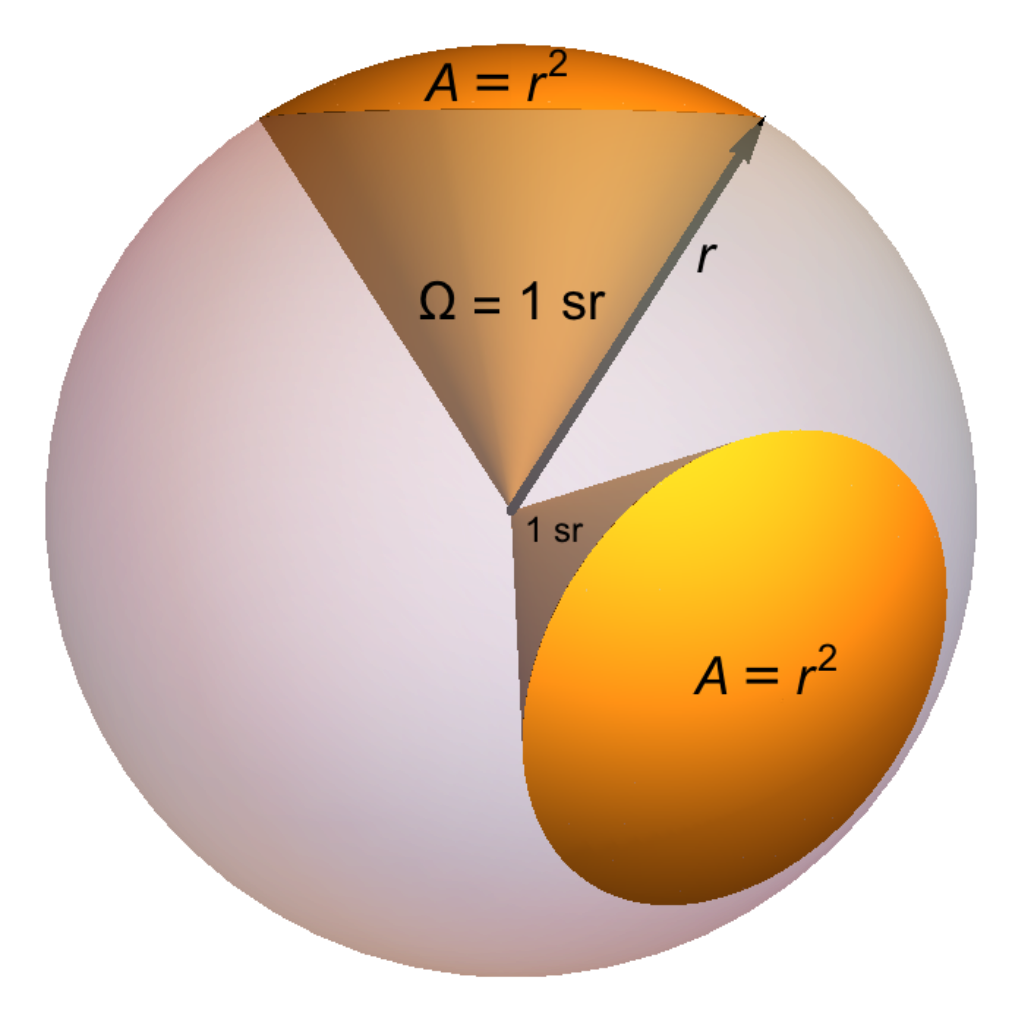
\includegraphics[width=0.25\textwidth]{../../figures/Solid_Angle_1_Steradian.png}\\
	\caption{Overview of 1 steradian. Credit: wikipedia}
	\label{fig:steradian}
      \end{figure}
      
    \subsubsection{Quantum efficiency}

    An overview of 
    
    \begin{figure}[H]
      \centering
      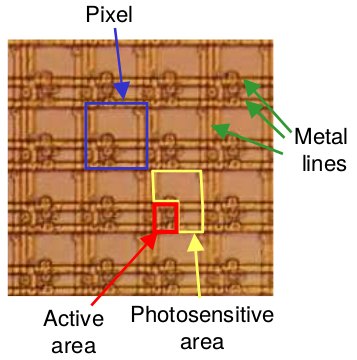
\includegraphics[width=0.25\textwidth]{../../figures/cmos_pixel_microscope.png}\\
      \caption{Microscope view of a cmos sensor surface, from \cite{Estribeau_2005}}
      \label{fig:cmos_pixel_microscope}
    \end{figure}
    
    \begin{figure}[H]
      \centering
      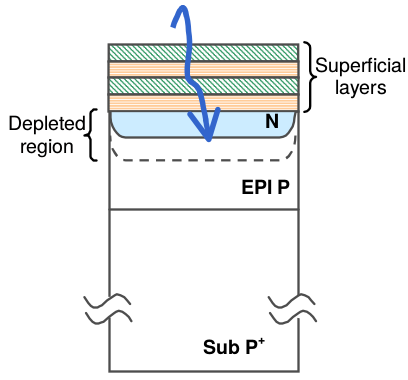
\includegraphics[width=0.25\textwidth]{../../figures/cmos_photodiode_cross_section.png}\\
      \caption{CMOS photodiode cross section schematic from \cite{Estribeau_2005}}
      \label{fig:cmos_photodiode_cross_section}
    \end{figure}

    
    \begin{figure}[H]
      \centering
      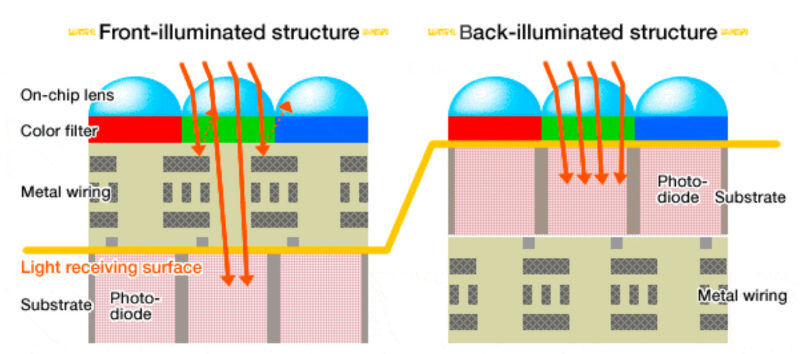
\includegraphics[width=0.5\textwidth]{../../figures/FSIvsBSI.png}\\
      \caption{Front side illuminated vs back side illuminated sensor, courtesy  \href{https://www.dtcommercialphoto.com/bsi-sensors-demystified/}{dtcommercialphoto.com}}
      \label{fig:fsi_vs_bsi}
    \end{figure}
    
    
    \subsubsection{Crosstalk}
     Another good introduction to what is crosstalk can be found in \cite{agranov2001crosstalk}, we hereby reproduce their definition:
     \blockquote{
     Crosstalk in an image sensor array degrades the spatial resolution, reduces overall sensitivity, makes poor color separation, and leads to additional noise in the image after color correction procedure. We will consider crosstalk in CMOS image sensors as consisting of three main components:
     \begin{itemize}
      \item Spectral crosstalk. This component is due to imperfect color filters passing through some amount of unwanted light of other colors.
      \item Optical spatial crosstalk. The main reason for this component of crosstalk is that color filters are located at some distance from the pixel surface due to metal and insulation layers. The light coming at angles other than orthogonal passes through a filter and can partially be absorbed by the adjacent pixel rather than one below. Depending on the f/d ratio of the lens, this portion of the light absorbed by neighboring pixel can vary significantly and can be big enough for low f/d ratios. micro-Lenses located on the top of color filters reduce this component of crosstalk significantly when appropriate form of micro-lenses and optimum position of them are chosen.
      \item Electrical crosstalk. This component of cross-talk results from photo-generated carriers having the possibility to move to neighboring charge accumulation sites. In comparison to the previous two components, this crosstalk occurs in both monochrome and color image sensors. The quantity of the carriers that can be accumulated by the neighboring pixel and the corresponding crosstalk strongly depends on the pixel structure, collection area, and distribution of sensitivity inside a pixel.
     \end{itemize}
      
      }
     Another good introduction to what is crosstalk, and how it can be caracterized in cmos sensors, can be found in \cite{Estribeau_2005}. Basically, we can retain than crosstalk is a short range interaction, that is wavelength dependant, see in particular one of the figure from \cite{Estribeau_2005} we reproduced in \ref{fig:estribeau_crosstalk_1}
     \begin{figure}[H]
      \centering
      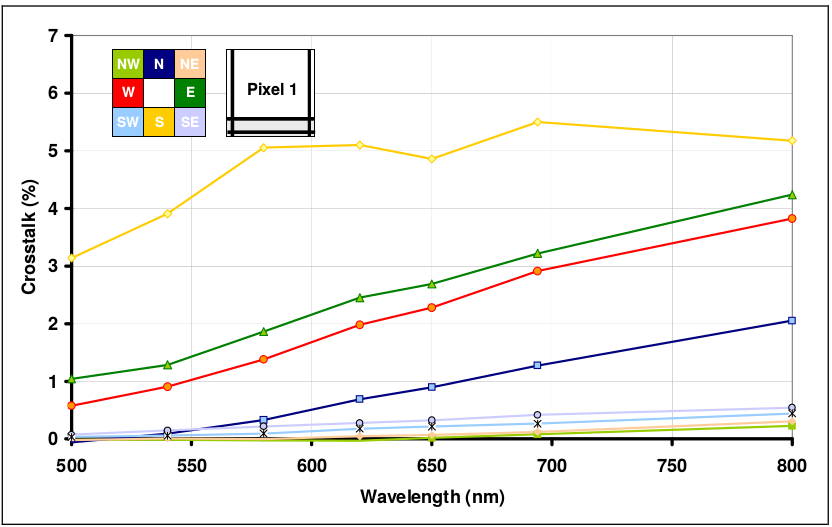
\includegraphics[width=0.75\textwidth]{../../figures/crosstalk_mono_ex1.png}\\
      \caption{Crosstalk measurment from a mono sensor in an experiment from \cite{Estribeau_2005} where all but central pixel are masked}
      \label{fig:estribeau_crosstalk_1}
     \end{figure}
     
     In this very interesting paper the author emphasize that the profile of the symmetry of the crosstalk is highly dependant on the shape and material of the active part (non sensitive) of the pixel surface. Hence the results might be different from one sensor to another.
  
     
    
  \subsection{Calibration system}
    \subsubsection{Spectrometer radiometric calibration}
    The are mainly two types of calibrations one can relatively easily perform with a quality spectrometer:
    \begin{itemize}
     \item \textbf{Spectral calibration}: The mapping between spectrometer numerical output bins (2048 bins on our model) and their corresponding wavelength. 
     \item \textbf{Irradiance calibration} The mapping between spectrometer numerical output values (digital counts) to an absolute value of spectral irradiance, expressed in $\mu W . cm^{-2} . nm^{-1}$.
    \end{itemize}

    The spectral mapping can be checked and fine tuned physically, turning knobs, by matching emission lines wavelength seen on acquisitions to a set of emission lines across UV/NIR from a known light source, made of Mercury and Argon in our case.
    
    The spectrometer used during our experiments as been also calibrated for spectral irradiance with a specifically deisgned light source, that is very stable (after a period of stabilization of 20 minutes) of known spectral irradiance. The output of the calibration process is a set of coefficient stored in a file, we call calibration coefficient values or $Coeff_{calibration}$. Each of those coefficient is homogeneous to $\mu J . cm^{-2}$
    
    The calibration procedure consists in applying the following equation over each acquisition:
    
    \begin{align*}
     Irr(i) = Reference(i) . \frac{ADU(i)-Dark(i)}{Exposure\_time * Exposed\_Area\_ratio * \Delta_{\lambda}(i)}
    \end{align*}

    where we have
    \begin{itemize}
     \item $Irr(i)$ is the scalar standing for the calibrated irradiance value at spectrometer bin index $i$. Its unit is $\mu W . cm^{-2} . nm^{-1}$
     \item $Coeff_{calibration}$ is the scalar standing for the calibration coefficient value at spectrometer bin index $i$. Its unit is $\mu J . cm^{-2}$
     \item $ADU(i)$ is the scalar standing for the actual digital count measured by the spectrometer
     \item $Dark(i)$ is the scalar standing for the baseline dark signal measurment made with the same exposure time as the current measure
     \item $Exposure\_time$ is the scalar standing for the exposure time of the acquisition in seconds
     \item $Exposed\_Area\_ratio$ is the scalar standing for the ratio in between surface exposed during calibration procedure, and the current measurment exposed area. If there is no vignetting or specific conditions reducing the physical light flux ending up on the spectrometer sensor, a ratio of 1 can be used.
     \item $\Delta_{\lambda}(i)$ is the scalar standing for the bandwidth of the spectrometer bin index $i$. It is expressed in $nm$
    \end{itemize}

    Once the output of the spectrometer have been calibrated, usually, one can integrate them over an arbitrary bandwidth, to obtain proper irradiance value in $\mu W . cm^{-2}$.
    
    \subsubsection{Integration sphere}

  \subsection{Pixel sensitivity and unit normalization modeling}
    In this section, we will present two approaches for modeling the process that leads to light flux being detected by the pixel's sensor in the camera. That accounts for , conversion from camera ADU to calibrated radiance, also accounting for vignetting and various sensor imperfections that can act on quantum efficiency eventually diminishing the available light flux depending on the area of the sensor and that is pixel dependent. We will also present approaches to model crosstalk in between neighbouring pixels.
    
    \subsubsection{Radiometric calibration unit normalization}
    As one can see from the definition of spectral irradiance integrated over a given bandwidth: $\mu W . cm^{-2}$ that values are instantaneous, or normalized per unit of time, as $W$ can be expressed as $J . s^{-1}$. As our calibration process involve image acquisition with different exposure time, we will simply need to first account for this difference in exposure.
    
    After being corrected for electronic calibration seen in previous section, we will simply apply to both camera acquisition, an exposure time normalization:
    
    \begin{align*}
     A_{tnorm} = \frac{1}{Et} A_{preprocessed} 
    \end{align*}

    where
    \begin{itemize}
     \item $A_{preprocessed}$ is the vector of preprocessed ADU counts seen in previous section, in unit ADU count
     \item $A_{tnorm}$ is the vector of exposure time normalized ADU counts, its unit would be $ADU/s$
     \item $Et$ is a scalar representing a frame exposure time in second.
    \end{itemize}

    
    \subsubsection{Pixel based sensitivity correction}
    As we want to obtain spectral radiance in unit of $\mu W . cm^{-2}$, independantly of whether input light flux is collimated or not. we are going ot use our integrating sphere to acquire reference images with various spectral patterns, and concurrently acquire spetra with our reference irradiance calibrated spectrometer pointed towards another output of the calibration sphere.
    
    We assume that our sensor values are already calibrated for linearity. Now we also assume that every interaction that leads to the overall light flux entering the camera optical system being decreased before being transformed into ADU count and then in radiometric flux can be modeled with a linear transform:
    
    \begin{align*}
     F_{i,j} = R{i,j} A_{tnorm_{i,j}}
    \end{align*}
    
    with
    \begin{itemize}
     \item $F_{i,j}$ is a scalar representing the actual irradiance measured by the pixels in $\mu W . cm^{-2}$ at pixel position $\{i,j\}$
     \item $A_{tnorm_{i,j}}$ is the ADU count actually measured by the sensor at pixel position $\{i,j\}$, normalized per exposure time.
     \item $R{i,j}$ is a scalar used as a scaling factor to convert from $ADU.s^{-1}$ to corresponding irradiance in $\mu W . cm^{-2}$ at pixel position $\{i,j\}$. Hence this coefficient should be homogeneous to $\mu J . cm^{-2} . ADU^{-1}$
    \end{itemize}

    As our sensor has already been calibrated for linearity, and the residual offset due flux independant signal (dark current) should have been removed in previous steps, it seems unnecessary for us here, to try to use an affine model, as we might end up trying to solve a problem prone to instability if there are too many parameters in the next section.

    \subsubsection{Crosstalk modeling}
    Crosstalk is a very sensitive topic, as its effects are very difficult to disantangle from individual pixel spectral response and actual spatial correlation in natural scenes spectra. The behaviour of crosstalk might also change depending on light flux incoming angle, and local behaviour...
    
    Eventually, one of the biggest obstacle to proper modeling of crosstalk we have found, is that it is impossible to send a calibration light pattern on the sensor whose incident footprint indicator on the sensor would be a well defined list of pixels where flux would be maximum, although other neighbouring pixels right next to the indicator would receive no direct incident light, light it was done in \cite{Estribeau_2005} within a microelectronic laboratory conditions.
    Without actual modification of the sensor, this setup is impossible to reproduce because of the very nature of light (electromagnetic wave) and our optical system, that acts as an inteferometer, hence producing a smooth point spread function (interference pattern) whose FWHM in practice is larger than a single pixel.
    
    Although it is very difficult to measure crosstalk directly without making some assumptions, like spectral response of individual pixels is perfectly consistent across the whole sensor, we can try to model it and see if we can eventually infer some informations about it.

    When reviewing the litterature, it appeared that microlenses on top of most of the sensors plays an important role in reducing the crosstalk. In particular, BSI sensors, that are known for their very high quantum efficiency, and sensitive area, close to 100\% of the surface of the sensor, are usually still equipped with microlenses. Here is what we can read about BSI and crosstalk in \cite{taverni2018front}:
    
    
    \blockquote{BSI still uses microlenses to direct the light to the photodiode and away from the other transitors. Microlenses also reduce optical cross-talk, as light coming in at a steep angle is less prone to end up in the neighboring pixel. This is particularly important for red light which passes through more silicon before being absorbed. Without microlenses, chromatic aberation would be worse.}
    
    

    \paragraph{Filter level contamination}
    The first model we can think of is a model where the amount of light that is measured on every pixel depends on incoming incident flux falling onto neighboring pixel, but its contribution to local considered pixel can be different from local or remote underlying pixel response.
    
    The model can be written with the following equality
    
    \begin{align*}
     \begin{pmatrix}
      0 \\
      1
     \end{pmatrix}
    \end{align*}

    
    
    \paragraph{Post filtering contamination}
    
    
    





%----------------------------------------------------------------------------------------
%	SECTION 3
%----------------------------------------------------------------------------------------

\section{Optical sensor calibration}
  \subsection{Definitions}
    \subsubsection{System point spread function}

  \subsection{System point spread function}
    \subsubsection{Measurment of PSF with articial star}
      Measuring the point spread function of an imaging system is functionally equivalent to measure the impulse response of a dynamical system, although the single temporal dimension is replaced by two spatial dimensions, and the concept of  causality does not really apply.
      There are mainly two ways to measure the impulse response of a system:
      \begin{itemize}
      \item Send an arbitrary known input signal/sequence, measure system output
      \end{itemize}

%----------------------------------------------------------------------------------------
%	SECTION 4
%----------------------------------------------------------------------------------------

\section{Camera}
  \subsection{Sensor features}

    \subsubsection{Introduction}
      XXXXX sensor is provided by a company called XXXX, that manufactures XXXXXXX on top of off the shelf
      cmos sensors. The original cmos sensor that XXX uses to build the XXX camera is the XXXX by XXXXXX:

      \begin{figure}[h!]
	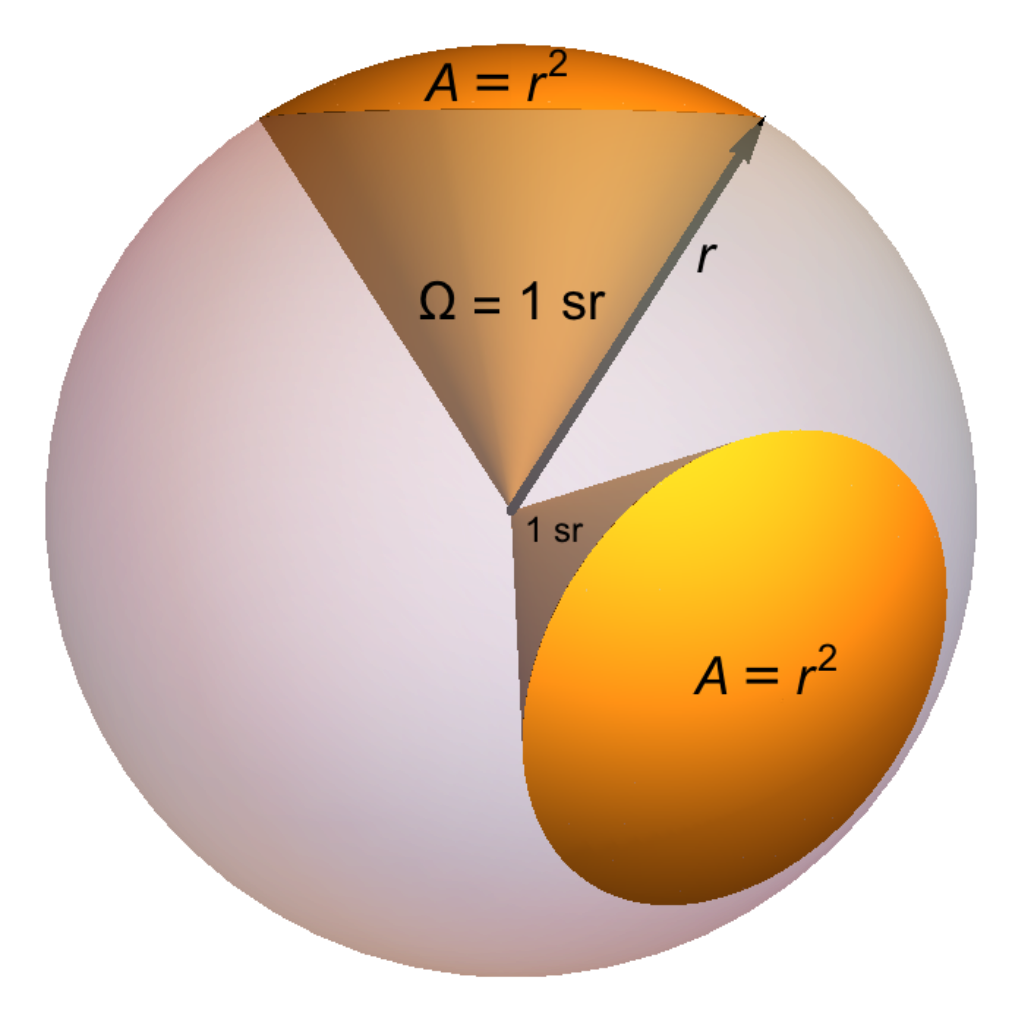
\includegraphics[width=1.0\textwidth]{../../figures/Solid_Angle_1_Steradian.png}\\
	\caption{Constructor picture of the stock CMV2000}
	\label{fig:stock_cmv_picture}
      \end{figure}

    \subsubsection{Constructor data}
      Here are the constructor data for the stock cmv2000 (before imec post processing)
      \begin{table}
	\centering
	\begin{tabular}{|l|l|l|l|}
	  \hline
	  \textbf{Parameter} & \textbf{Value} & \textbf{unit} & \textbf{comment}\\
	  \hline
	    Resolution & $2048 \times 1088$ & & Useful pixels \\
	    Sensor size & $11.264 \times 5.984$ & mm & Rectangular sensor \\
	    Pixel pitch & $5.5 \times 5.5$ & $\mu m$ & Pixels are square \\
	    Bit depth & 8 - 10 - 12 & bits & depends on adc resolution\\
	    Full well charge & $13500$ & e- & \\
	    Dark current & 125 & e-/s & (@ 25°C die temperature) \\
	    Dark current associated noise & 13 & e- & RMS value \\
	    Conversion gain & 0.075 & LSB/e- & (10 bit mode) at unity gain\\
	    Parasitic light sensitivity & 1/50000 & & \\
	    Dynamic range & 60 & dB & \\
	    Power consumption & 650 & mW & \\
	    Fixed pattern noise & <1 & LSB & 10 bit mode, <0.1\% of full swing, standard deviation on full image) \\
	  \hline
	\end{tabular}
	\caption{Stock cmv2000 sensor features}
	\label{tab:stock_cmv_features}
      \end{table}

    \subsubsection{Quantum efficiency}
      XXXX, the manufacturer of the XXXX cmos sensor provides a quantum efficiency curve for its stock sensor, that
      we reproduce here in figure \ref{fig:reference_to_qe_sensor}.
      We also put on the same figure, the actual measurments made by XXXX on the XXXX sensor. The drop in quantum efficiency is quite substancial, especially in the red, and NIR parts of the spectrum. We believe that part of this drop can be explained by XXXX internal process, where they eventually interfere with the microlenses that equips the xxx sensor, but there are also probably other factor, that we are still expecting XXXX to provide (point of contact: Klaas.Tack@XXXX.be)

      \begin{figure}[h!]
	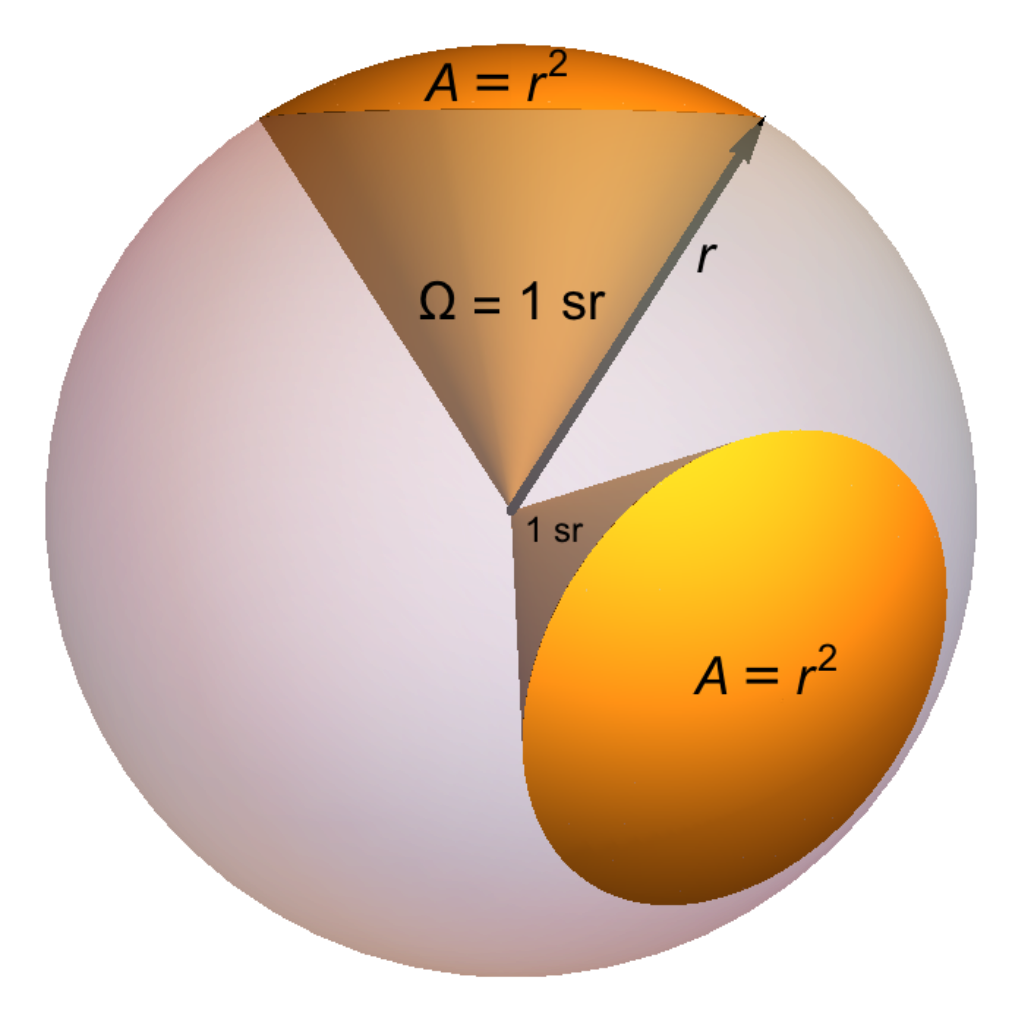
\includegraphics[width=1.0\textwidth]{../../figures/Solid_Angle_1_Steradian.png}\\
	\caption{Stock XXXXX constructor datasheet quantum efficiency}
	\label{fig:stock_xxx_qe}
      \end{figure}
      \begin{figure}[h!]
	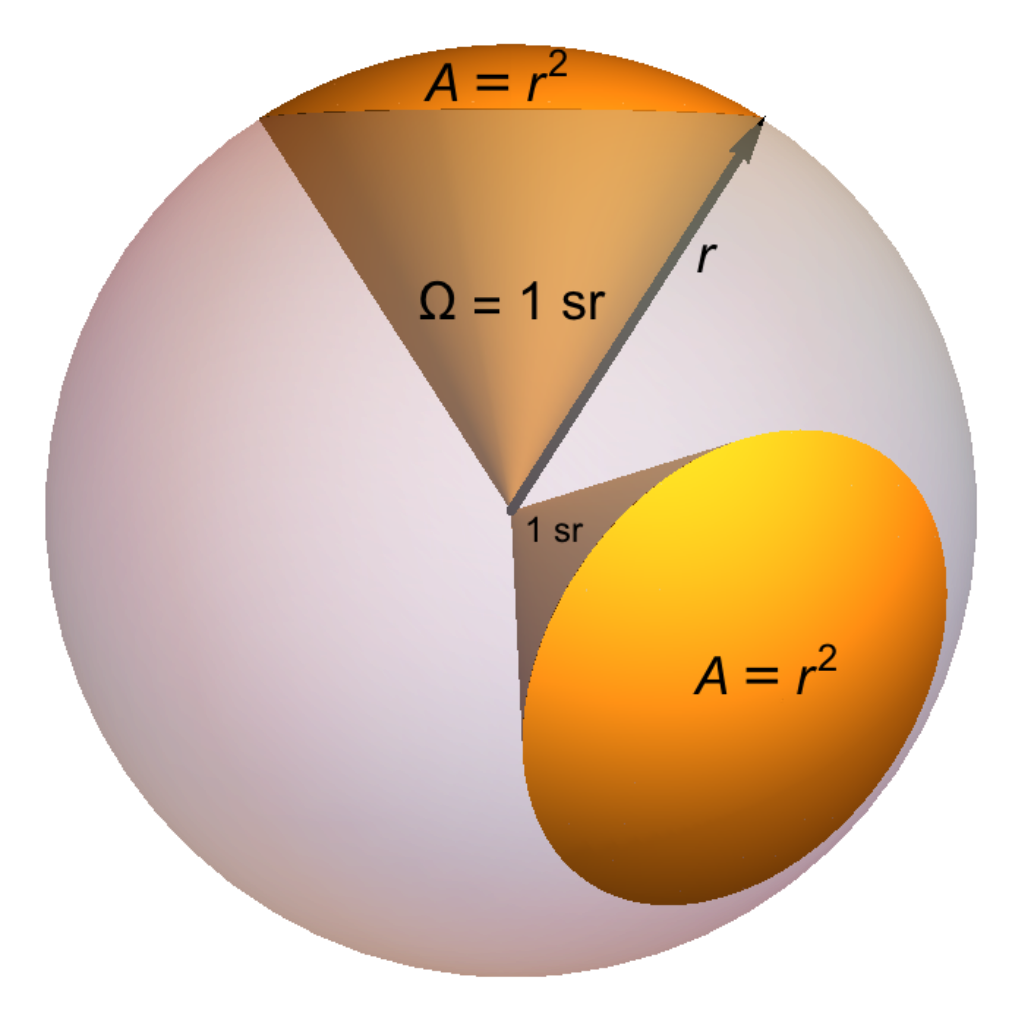
\includegraphics[width=1.0\textwidth]{../../figures/Solid_Angle_1_Steradian.png}\\
	\caption{XXXX sensor actual quantum efficiency, as measured per XXXX with colimated light.}
	\label{fig:reference_to_qe_sensor}
      \end{figure}

      \begin{figure}[h!]
	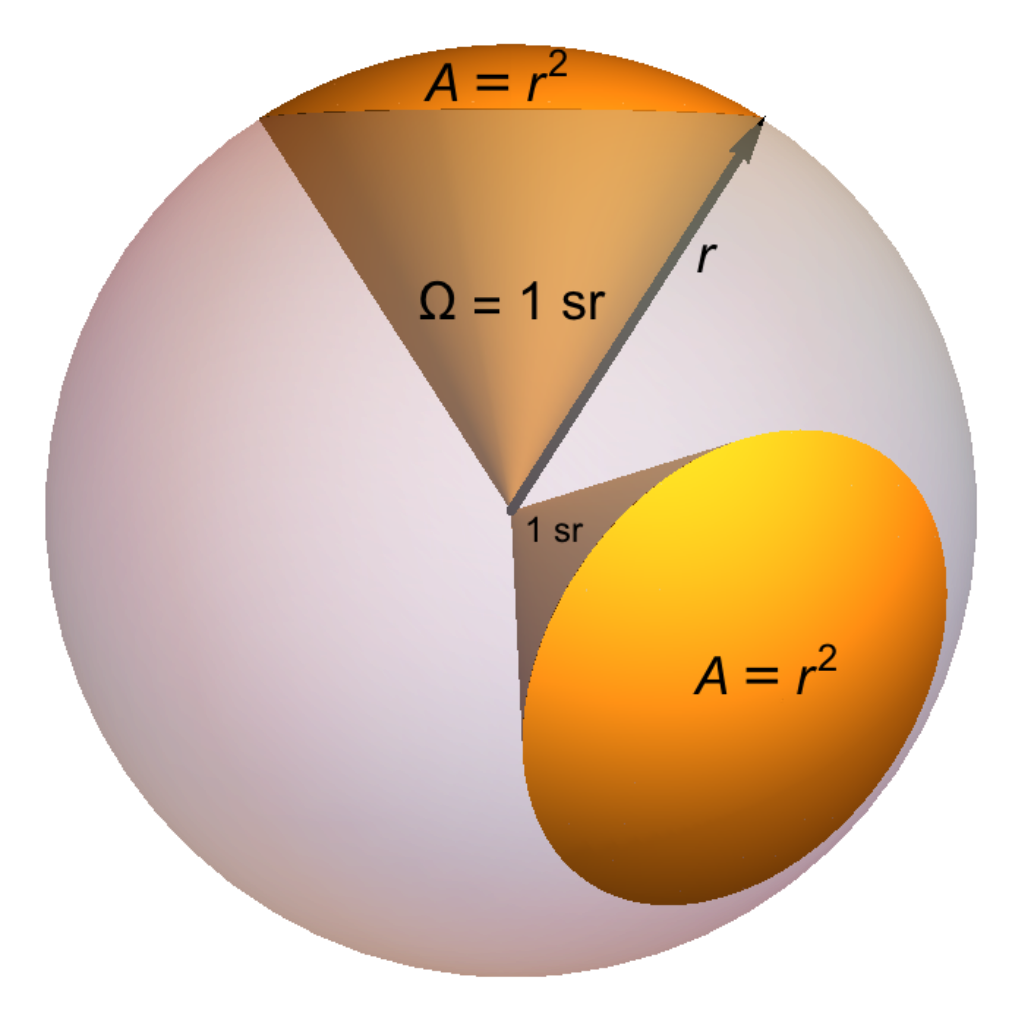
\includegraphics[width=1.0\textwidth]{../../figures/Solid_Angle_1_Steradian.png}\\
	\caption{XXXX sensor actual quantum efficiency}
      \end{figure}
      \begin{figure}[h!]
	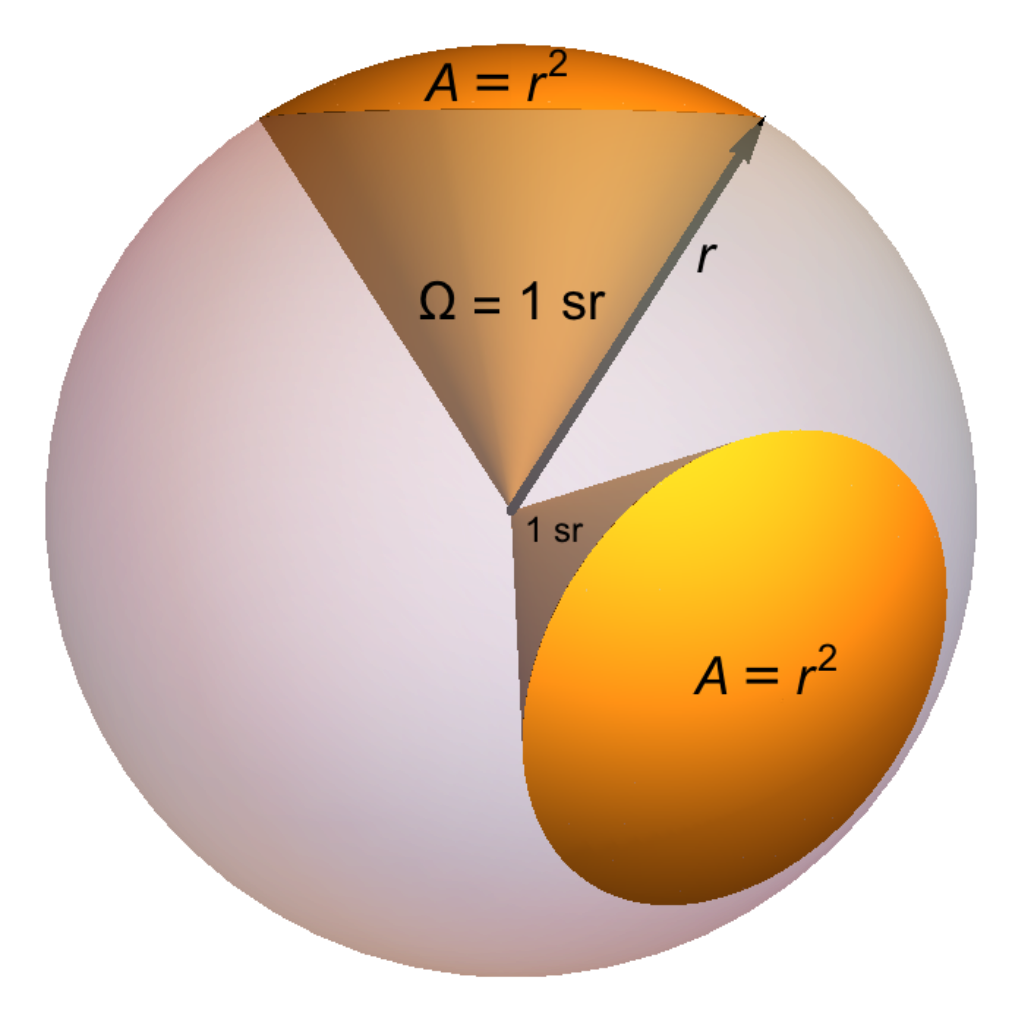
\includegraphics[width=1.0\textwidth]{../../figures/Solid_Angle_1_Steradian.png}\\
	\caption{XXXX sensor actual quantum efficiency}
      \end{figure}


      \begin{figure}[h!]
	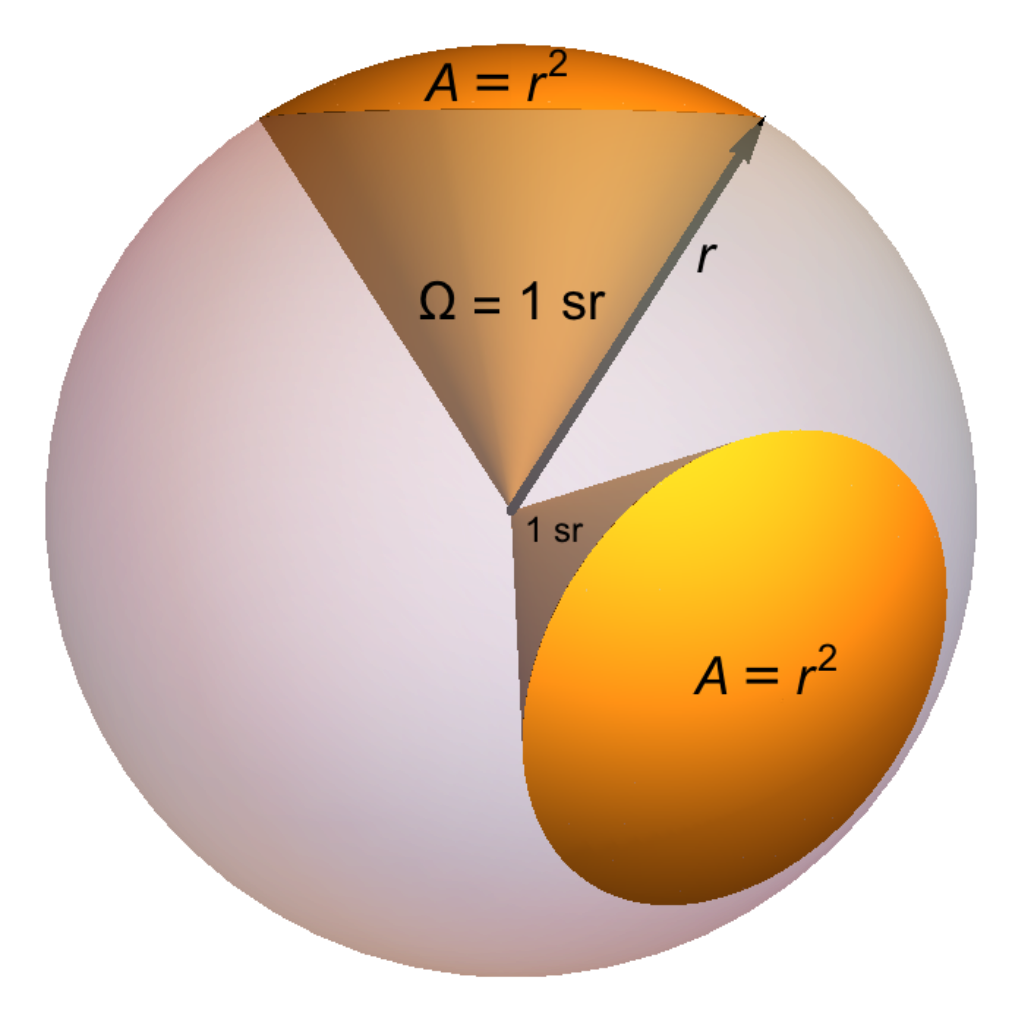
\includegraphics[width=1.0\textwidth]{../../figures/Solid_Angle_1_Steradian.png}\\
	\caption{XXXX sensor actual quantum efficiency}
      \end{figure}
      \begin{figure}[h!]
	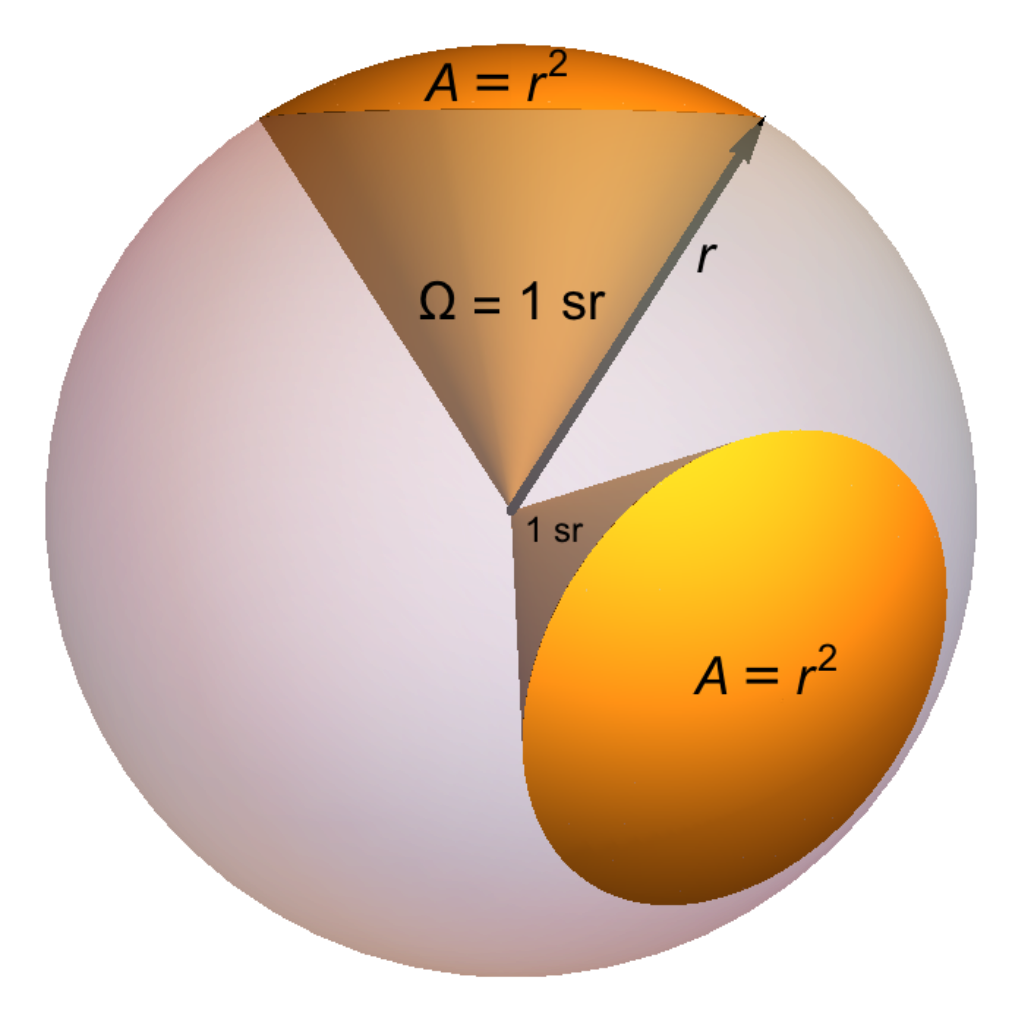
\includegraphics[width=1.0\textwidth]{../../figures/Solid_Angle_1_Steradian.png}\\
	\caption{XXXX sensor actual quantum efficiency}
      \end{figure}

        \subsection{Lens features}
    \subsubsection{Constructor data}
    diameter:
    focal:
    F/D ratio:
    optical design: number of lens
    Known aberration:
    Resulting theoretical system panchromatic system sampling scheme.

  \subsection{Cutoff filters}
  In order to avoid contamination of signal of interest by electromagnetic signal outside of the spectral window for which we target accurate radiometric calibration, we are using a combination of longpass and shortpass optical filters.

  The transmission curve:
  \begin{figure}[h!]
    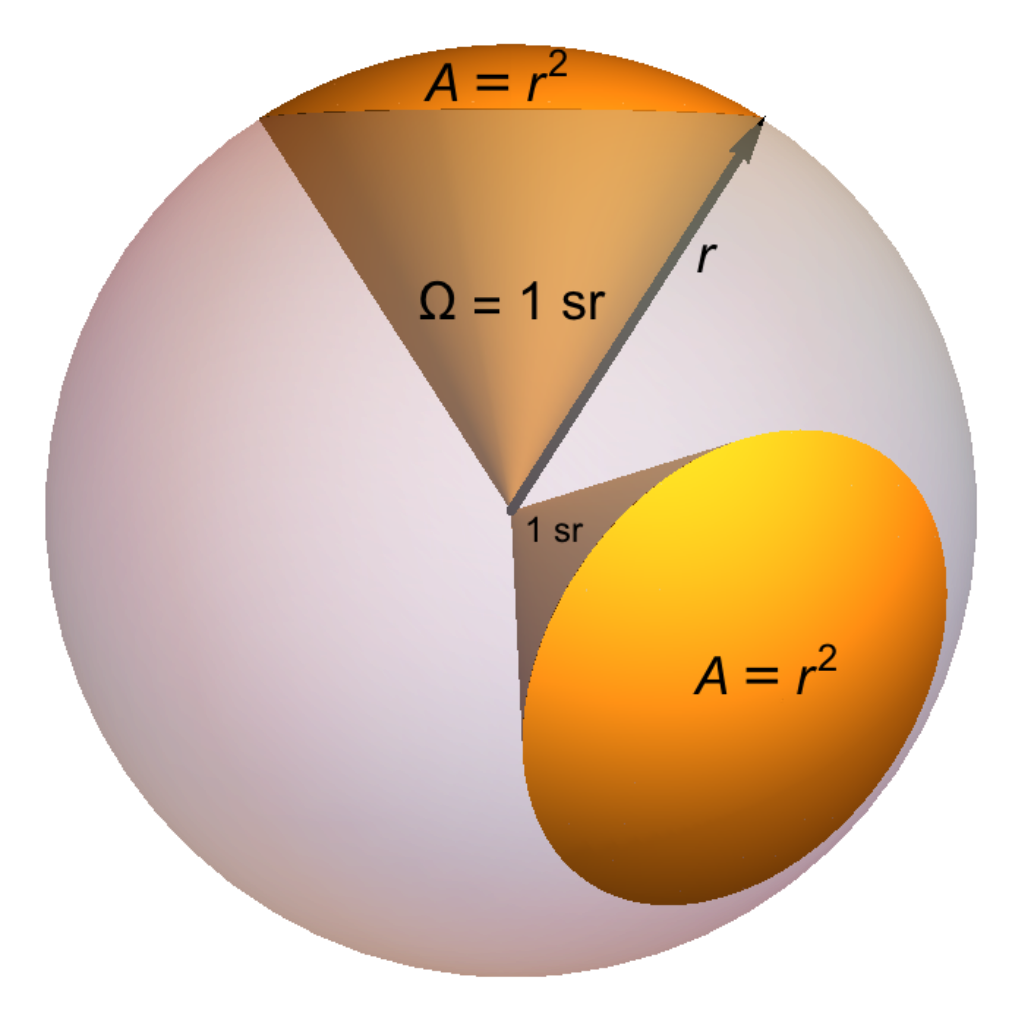
\includegraphics[width=1.0\textwidth]{../../figures/Solid_Angle_1_Steradian.png}\\
    \caption{Longpass optical filter transmission profile}
  \end{figure}


  The blocking curve:
  \begin{figure}[h!]
    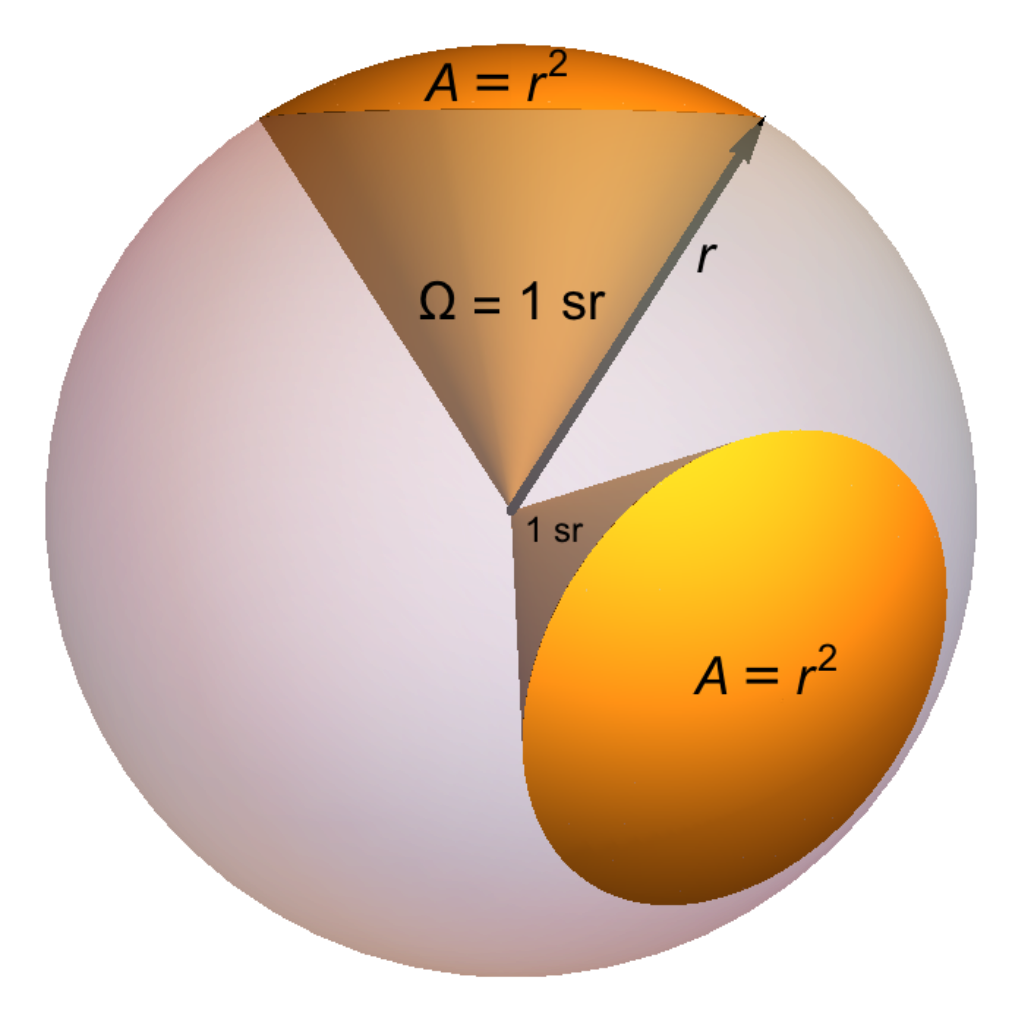
\includegraphics[width=1.0\textwidth]{../../figures/Solid_Angle_1_Steradian.png}\\
    \caption{Longpass optical filter blocking profile}
  \end{figure}

  \subsubsection longpass filter

  The transmission curve:
  \begin{figure}[h!]
    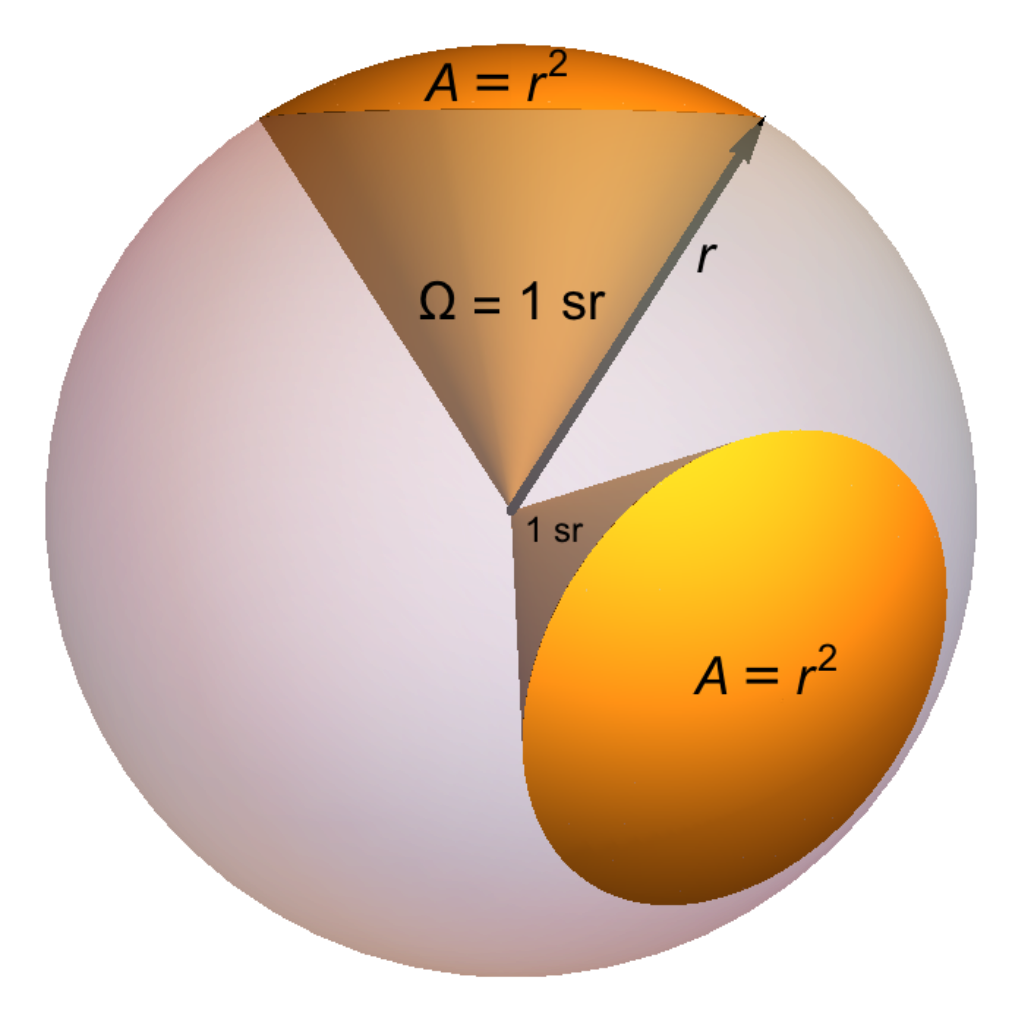
\includegraphics[width=1.0\textwidth]{../../figures/Solid_Angle_1_Steradian.png}\\
    \caption{Longpass optical filter transmission profile}
  \end{figure}


  The blocking curve:
  \begin{figure}[h!]
    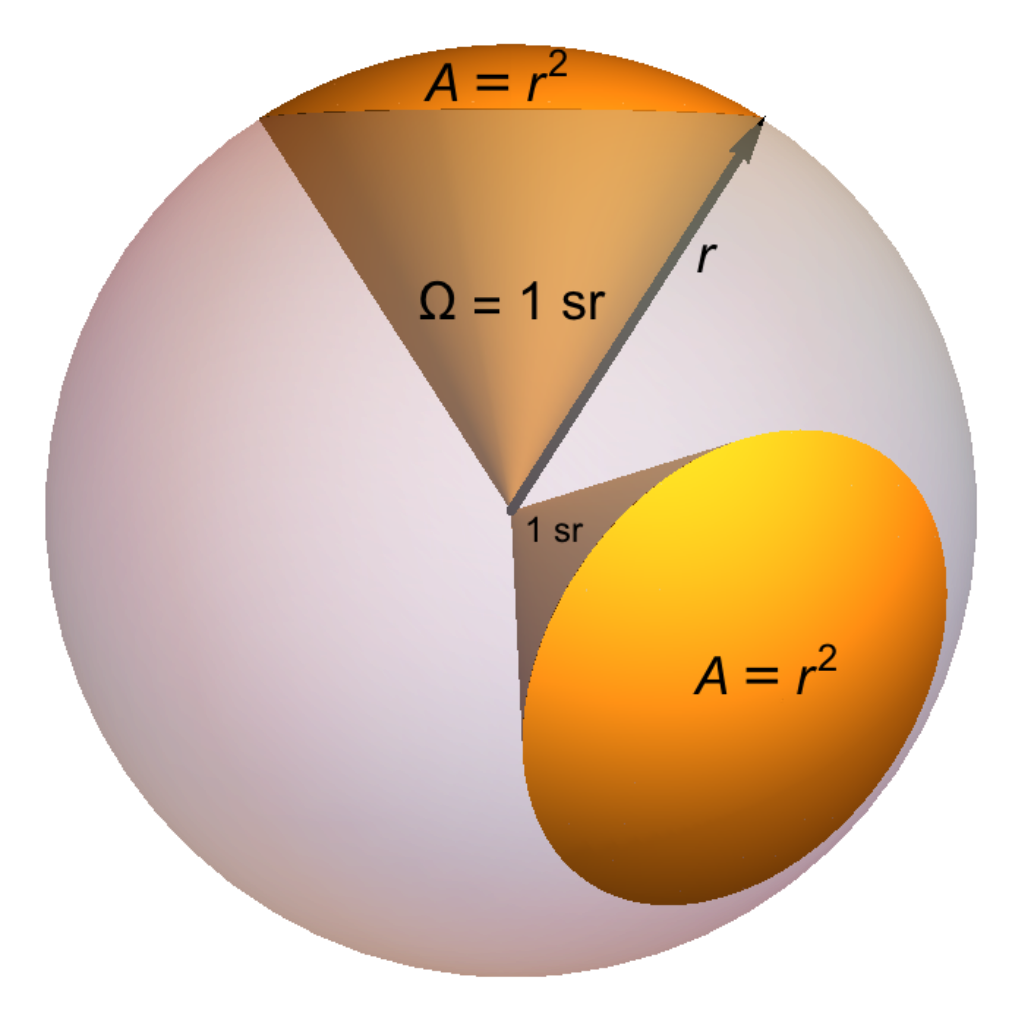
\includegraphics[width=1.0\textwidth]{../../figures/Solid_Angle_1_Steradian.png}\\
    \caption{Longpass optical filter blocking profile}
  \end{figure}


  \subsection{System calibration}
    \subsubsection{Sensor offset}
    offset map,
    \subsubsection{Sensor dark current}
    dark current table at different temperature and different gain
    Spatial correlation / search for Amp glow

    \subsubsection{Sensor linearity}
    affine regression parameters map per gain value

    \subsubsection{Sensor defect mapping}
    Detect outliers on linearity map

    \subsubsection{System point spread function}
      \paragraph{Measurment of PSF with articial star}
      Measuring the point spread function of an imaging system is functionally equivalent to measure the impulse response of a dynamical system, although the single temporal dimension is replaced by two spatial dimensions, and the concept of  causality does not really apply.
      There are mainly two ways to measure the impulse response of a system:
      \begin{itemize}
      \item Send an arbitrary known input signal/sequence, measure system output
      \end{itemize}

  \subsubsection{Global MTF per band}


%----------------------------------------------------------------------------------------
%	SECTION 5
%----------------------------------------------------------------------------------------

\section{Adequacy between imaging system and spectroscopy}

\begin{figure}[h!]
  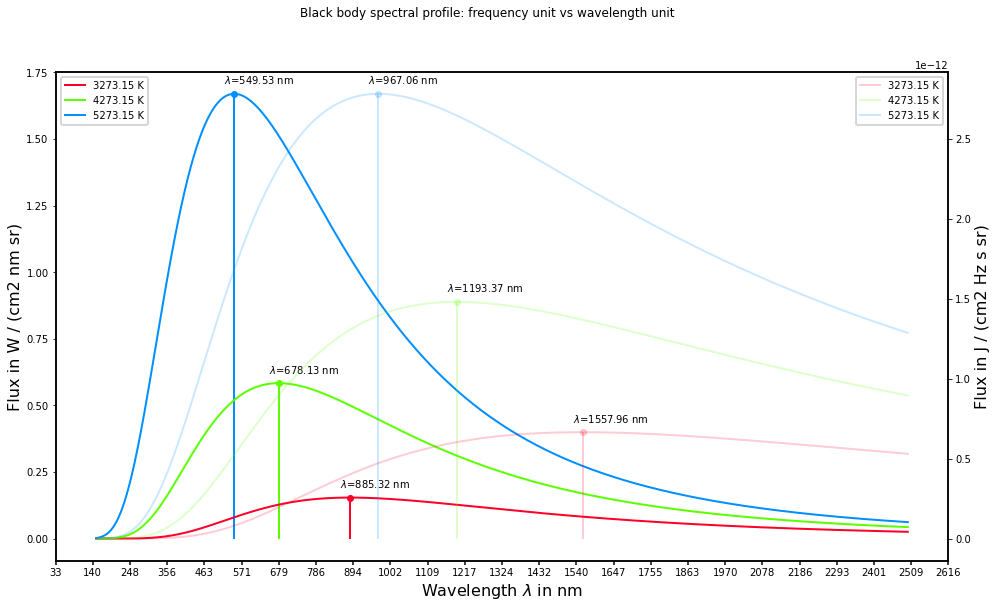
\includegraphics[width=1.0\textwidth]{../../figures/black_body_planck.png}\\
  \caption{Black body emissions}
\end{figure}

%----------------------------------------------------------------------------------------
%	SECTION 5
%----------------------------------------------------------------------------------------

\section{Results and Conclusions}



%----------------------------------------------------------------------------------------
%	BIBLIOGRAPHY
%----------------------------------------------------------------------------------------

\printbibliography

%----------------------------------------------------------------------------------------


\end{document}
